\chapter{Implementation}
This section deals with the realization of technical specification, design, software component and the standard algorithm. It includes methods which are implementations of those methods specified by the interface.

% ===================================================================================================
% TOOLS AND TECHNOLOGIES
% ===================================================================================================

\section{Tools and Technologies}

\subsection{NodeJS}

NodeJS\cite{NodeJS} is an open-source, cross-platform JavaScript run-time environment that executes JavaScript code server-side. Historically, JavaScript was used primarily for client-side scripting, in which scripts written in JavaScript are embedded in a webpage's HTML and run client-side by a JavaScript engine in the user's web browser. Node.js lets developers use JavaScript to write command line tools and for server-side scripting—running scripts server-side to produce dynamic web page content before the page is sent to the user's web browser. Consequently, Node.js represents a "JavaScript everywhere" paradigm, unifying web application development around a single programming language, rather than different languages for server side and client side scripts. 

NodeJS has been used to write the complete back-end of our mini-project for creating RESTful APIs that are used to integrate back-end with the front.  

NodeJS seemed an obvious choice given its popularity and well-built support. Use of NodeJS as back-end kept us close to our old programming methods without having to go deeper into the JS language in itself and also since it uses a faster v8 engine, it seemed a perfect fit to our craving for speed. 

\subsection{MongoDB}

The database used for this project is MongoDB\cite{MongoDB} which is a free and open-source cross-platform document-oriented database program. MongoDB uses JSON-like documents with schemas and is classified as a NoSQL database. It is published under a combination of the GNU Affero General Public License and the Apache License.

MongoDB is well-known for its no-SQL approach which was what we were looking for. MongoDB naturally lends itself to scalability and ease of use. It has a very good driver (mongoose) support which again makes it a good option. So our need is easily fulfilled using this database as it stores data in document format using key-value pairs and JS also works on JSON objects, thus simplifying the task of retrieving and manipulating the data.

\subsection{ReactJS}
ReactJS\cite{ReactJS} is a javascript library which is used for creating user interfaces. React makes it easy to maintain the front-end. As our project is a modular based project where all the features have been implemented as different modules, react, which uses a component-based approach to developing user interfaces, can go hand-in-hand with the back-end. Due to this very nature of React, we can easily scale it in future too. Moreover, react is very lightweight thus takes less loading time. Hence, it’s really convenient for designing our project’s user Interface.


% ===================================================================================================
% CODING STANDARDS FOLLOWED
% ===================================================================================================

\section{Coding Standards Followed}

\subsection{Proper Indentation / Structure}
The entire code is properly indented with uniform spaces and also leaving spaces between operands and operators. All the modules to be imported are imported at the top of the files, thus making the code clearer and easy to understand.

\subsection{Naming Convention}
The variables are given meaningful names and naming is performed using camel case variable naming convention. This makes the code neater and the code becomes more meaningful and easy to understand.

\subsection{Avoiding Callback Hell}
All the functions written inside the controller are designed using the async-await approach using promises, thus avoiding callbacks almost completely. This makes the code much more linear avoiding the deeply nested structure which results due to using callbacks, called the callback hell. We have successfully avoided that problem by writing all the functions using the async-await approach.

\subsection{Modular Approach}
Each feature has been implemented as a completely independent function which is exported by the controller module. The functioning of each and every one of these functions does not depend on or affect the functioning of other functions. This makes the addition and removal of new features easy. Also, debugging has been made easy due to this approach.

\subsection{Proper Folder Structure/Naming}
A standard folder structure has been followed in the project, keeping all the related files in different folders. The files containing the core functions are kept inside the controller folder, all the API end-point containing files are kept inside the routes folder, all the database schema models are kept inside the model's folder.

\subsection{Model View Controller Model}
Model–View–Controller (usually known as MVC) is an architectural pattern commonly used for developing user interfaces that divides an application into three interconnected parts. This is done to separate internal representations of information from the ways information is presented to and accepted from the user. The MVC design pattern decouples these major components allowing for efficient code reuse and parallel development.

\subsection{Documentation}
All the API end-points have been properly documented to make the integration easier and clear. The documentation contains the type of request to be sent to a specified route along with all the required input and the expected output along with all the constraints and error possibilities.

\pagebreak

% ===================================================================================================
% EXECUTION RESULTS AND DISCUSSIONS
% ===================================================================================================

\section{Execution Results and Discussions}

This section shows the execution results after integration and deployment. We shall be looking at some of the screenshots of the user interface which will outline the functioning of our app.


\begin{figure}[h!]
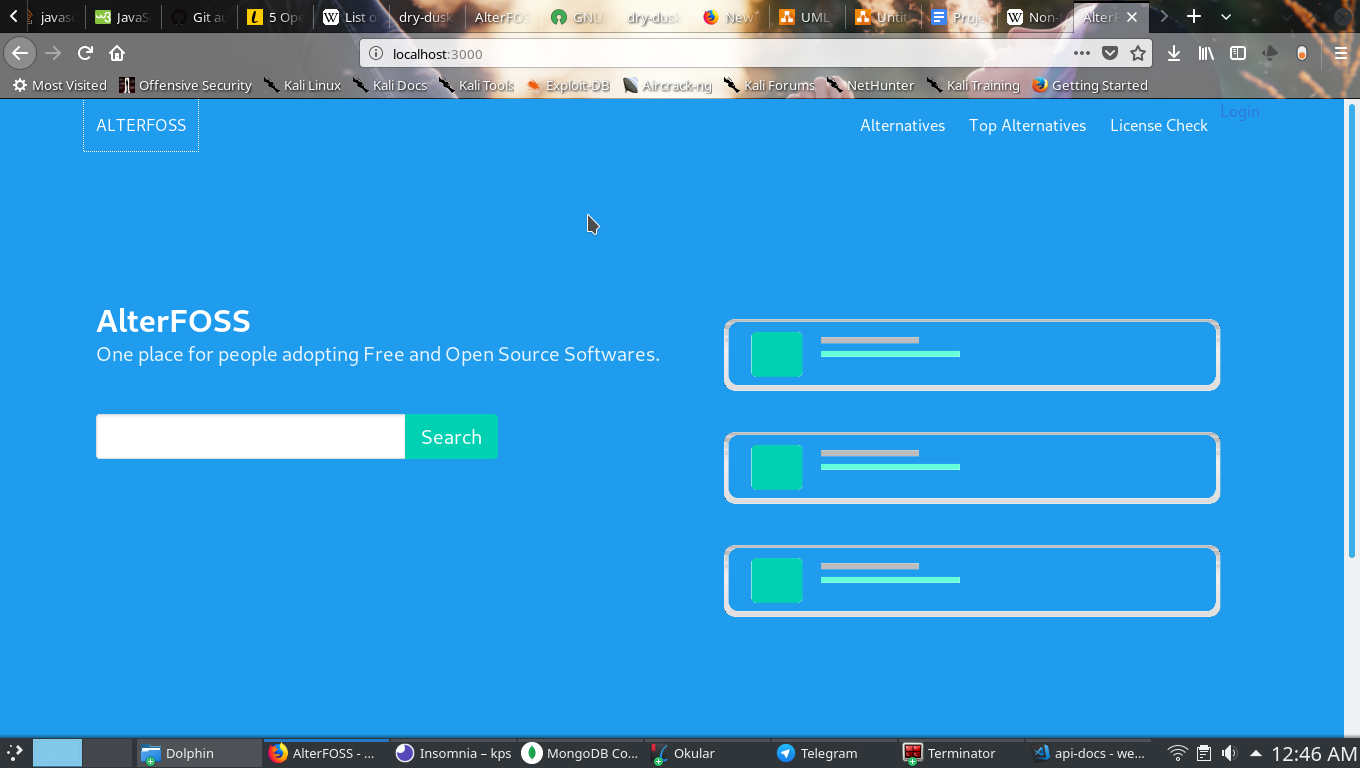
\includegraphics[scale=0.45]{images/4-1.png}
\caption{Home Page}
\label{fig:home_page}
\end{figure}


Figure \ref{fig:home_page} is the home page of our Web Application. The various links can be seen above such as alternatives to getting alternatives for proprietary softwares, top alternatives which are used to list out the top 10 alternatives based on upvotes. License check is used to check the license information of alternatives. The search bar shown here is used to search proprietary softwares based on the text the user passes via this text box.


\begin{figure}[h!]
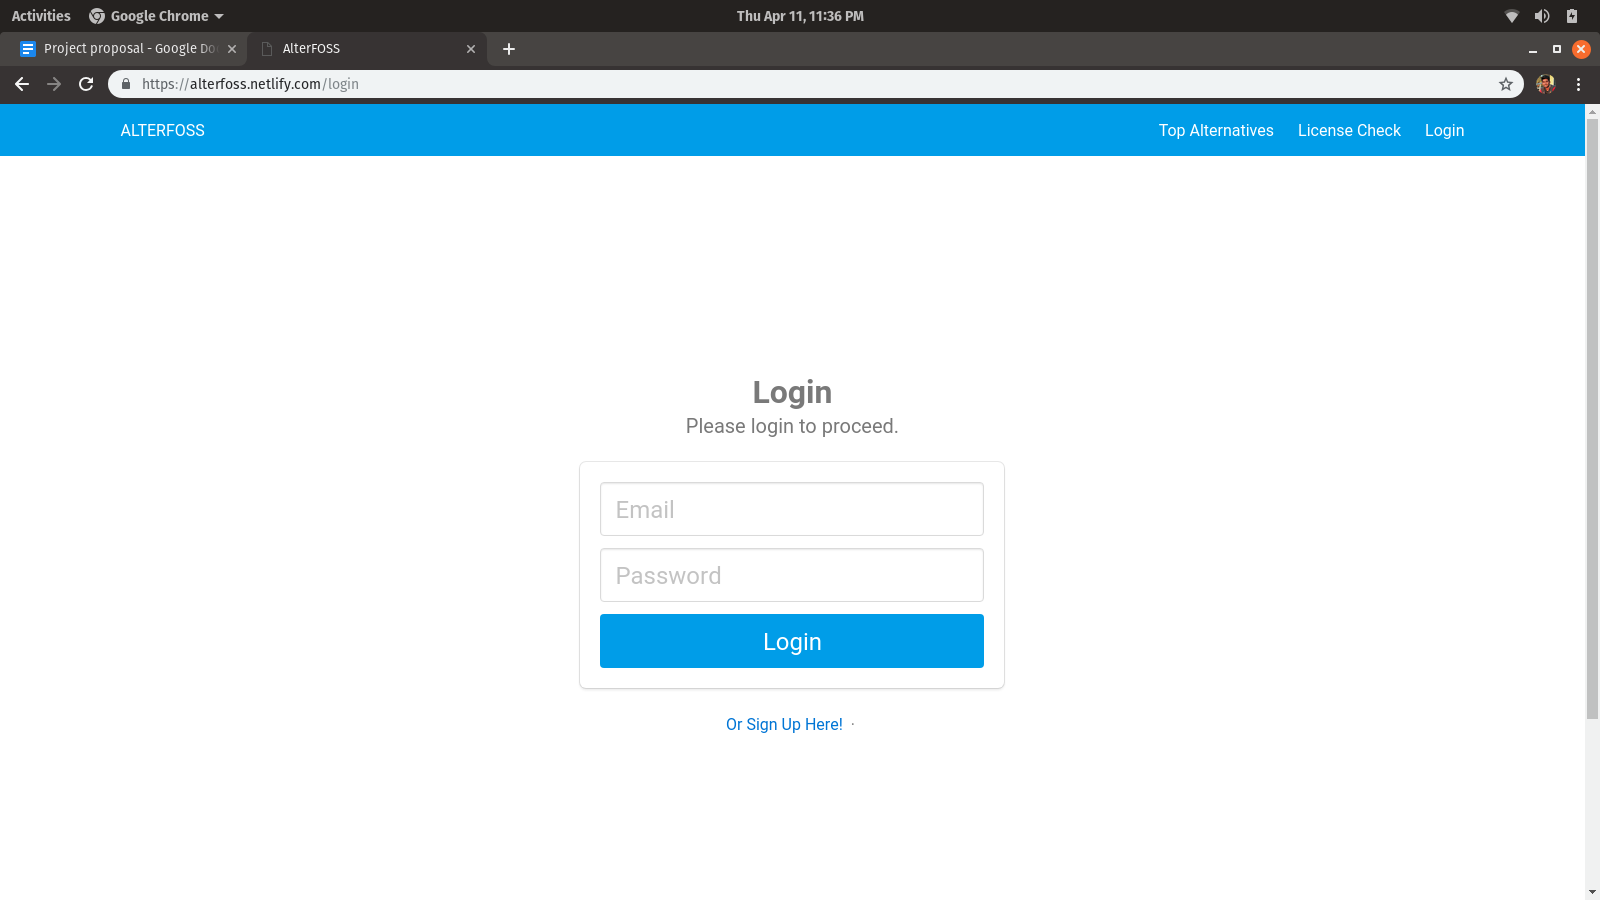
\includegraphics[scale=0.29]{images/login.png}
\caption{Login Page}
\label{fig:login_page}
\end{figure}

\begin{figure}[h!]
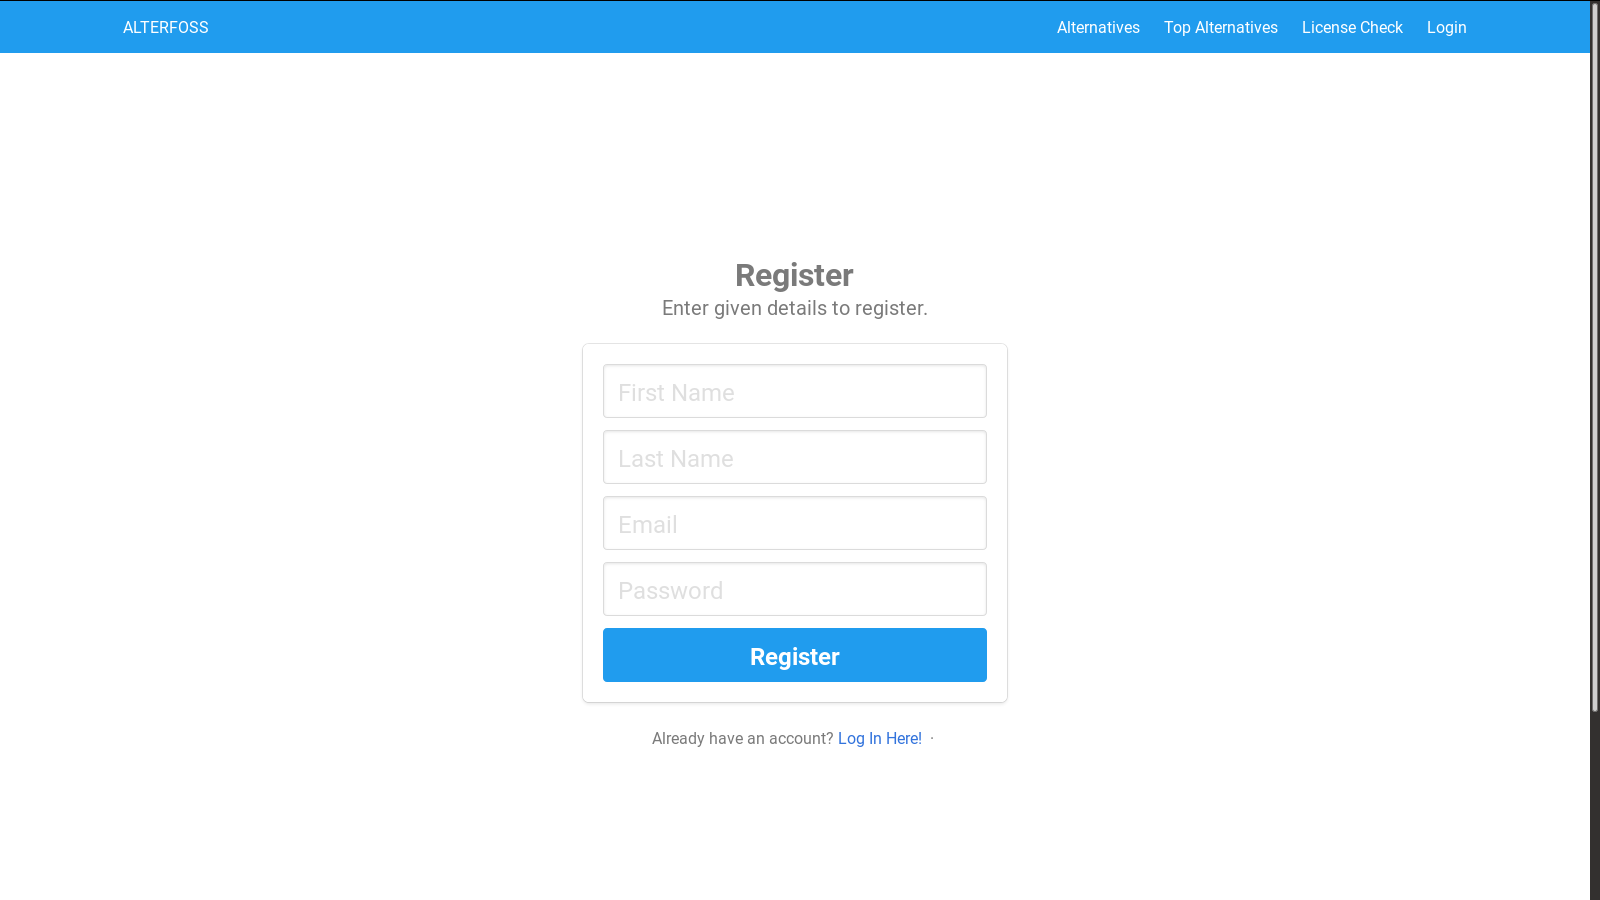
\includegraphics[scale=0.29]{images/register.png}
\caption{Home Page}
\label{fig:register_page}
\end{figure}

Figure ~\ref{fig:login_page} and Figure ~\ref{fig:register_page} show the authentication interfaces of the application.


\begin{figure}[h!]
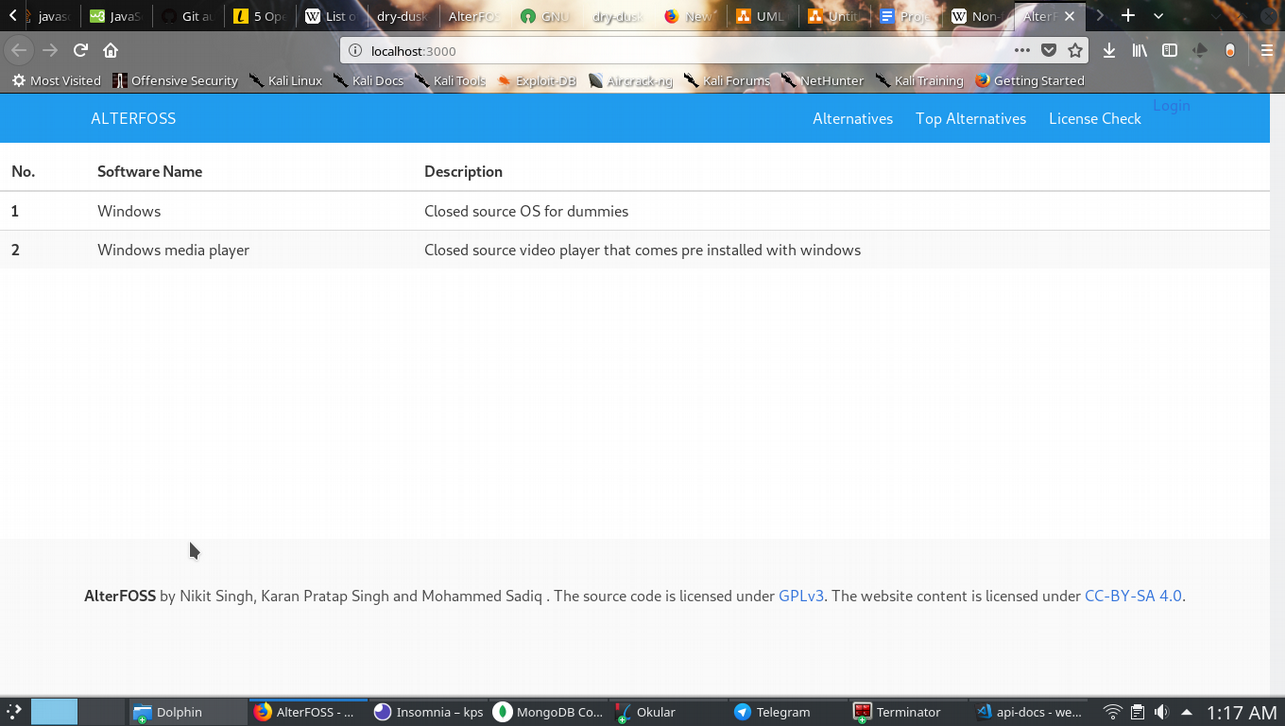
\includegraphics[scale=0.45]{images/4-2.png} 
\caption{Proprietary Search Results}
\label{fig:prop_srch_results}
\end{figure}

In Figure ~\ref{fig:prop_srch_results}, we had searched for 'windows media player' and those were the replies we got.

\begin{figure}[h!]
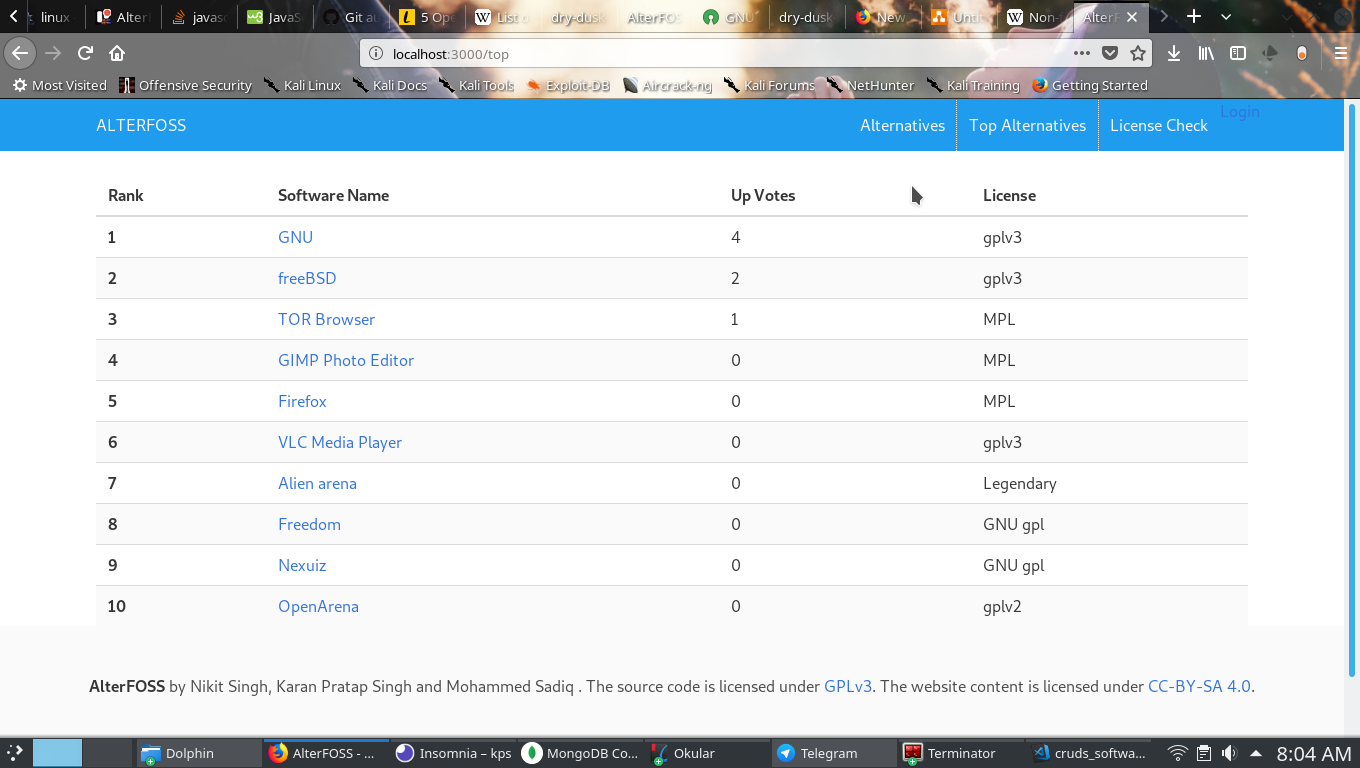
\includegraphics[scale=0.43]{images/4-3.png}
\caption{Top 10 alternatives}
\label{fig:top_ten_alt}
\end{figure}

As shown in Figure ~\ref{fig:top_ten_alt}, the top 10 alternatives list can be viewed by the user by clicking on the top alternatives option on the top right of the web page. It will display the list of top 10 alternatives along with their upvotes and license. This list is sorted, as discussed previously, based on the number of upvotes of the software. The API fetches the top 10 alternatives from the database, sorts them and sends them to the front end for display.


\begin{figure}[h!]
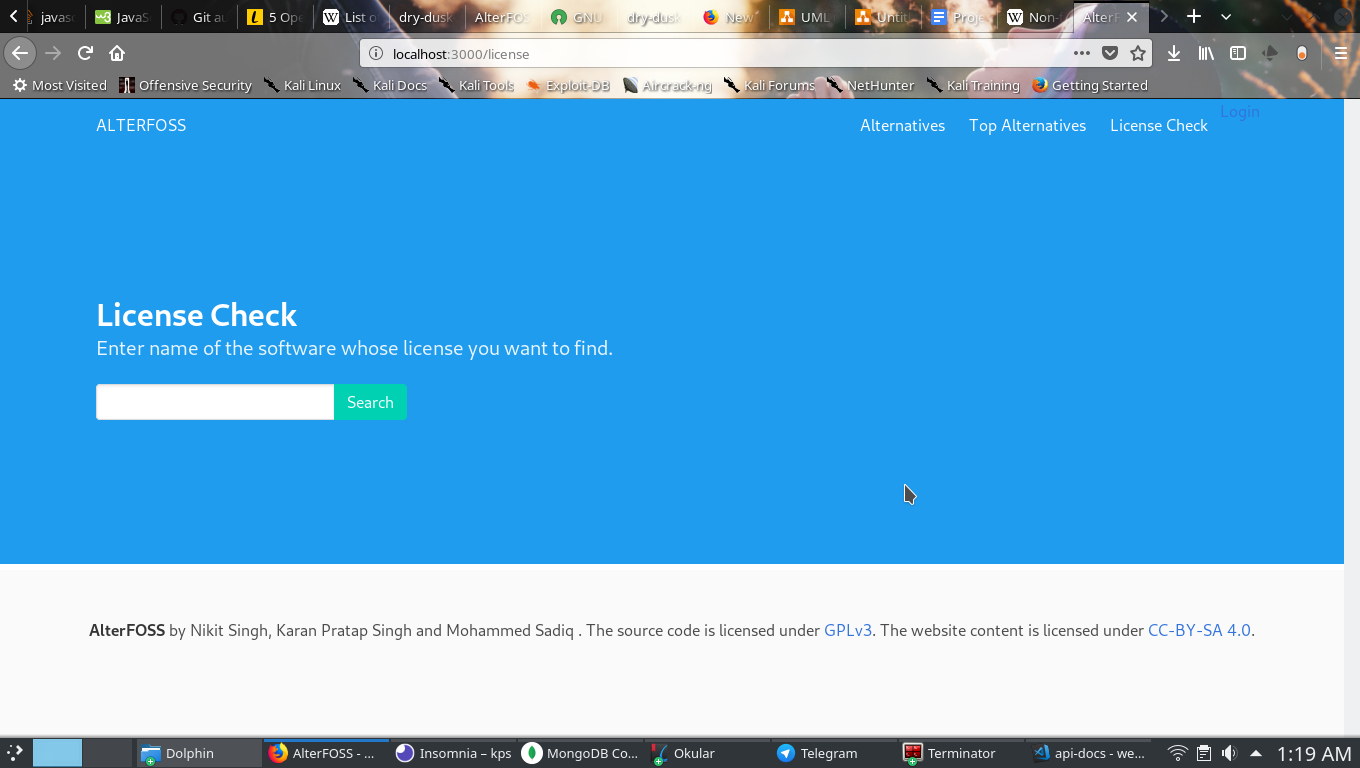
\includegraphics[scale=0.44]{images/4-4.png}
\caption{License Checker}
\label{fig:license_chk}
\end{figure}

Figure ~\ref{fig:license_chk} is the license checker module implemented in our mini project. The user can provide search text in the given text box to search alternative softwares. The result will be the name of the alternatives matching this search string along with their license information. Thus, the user can get the license information of any proprietary software he desires using this module.

\begin{figure}[h!]
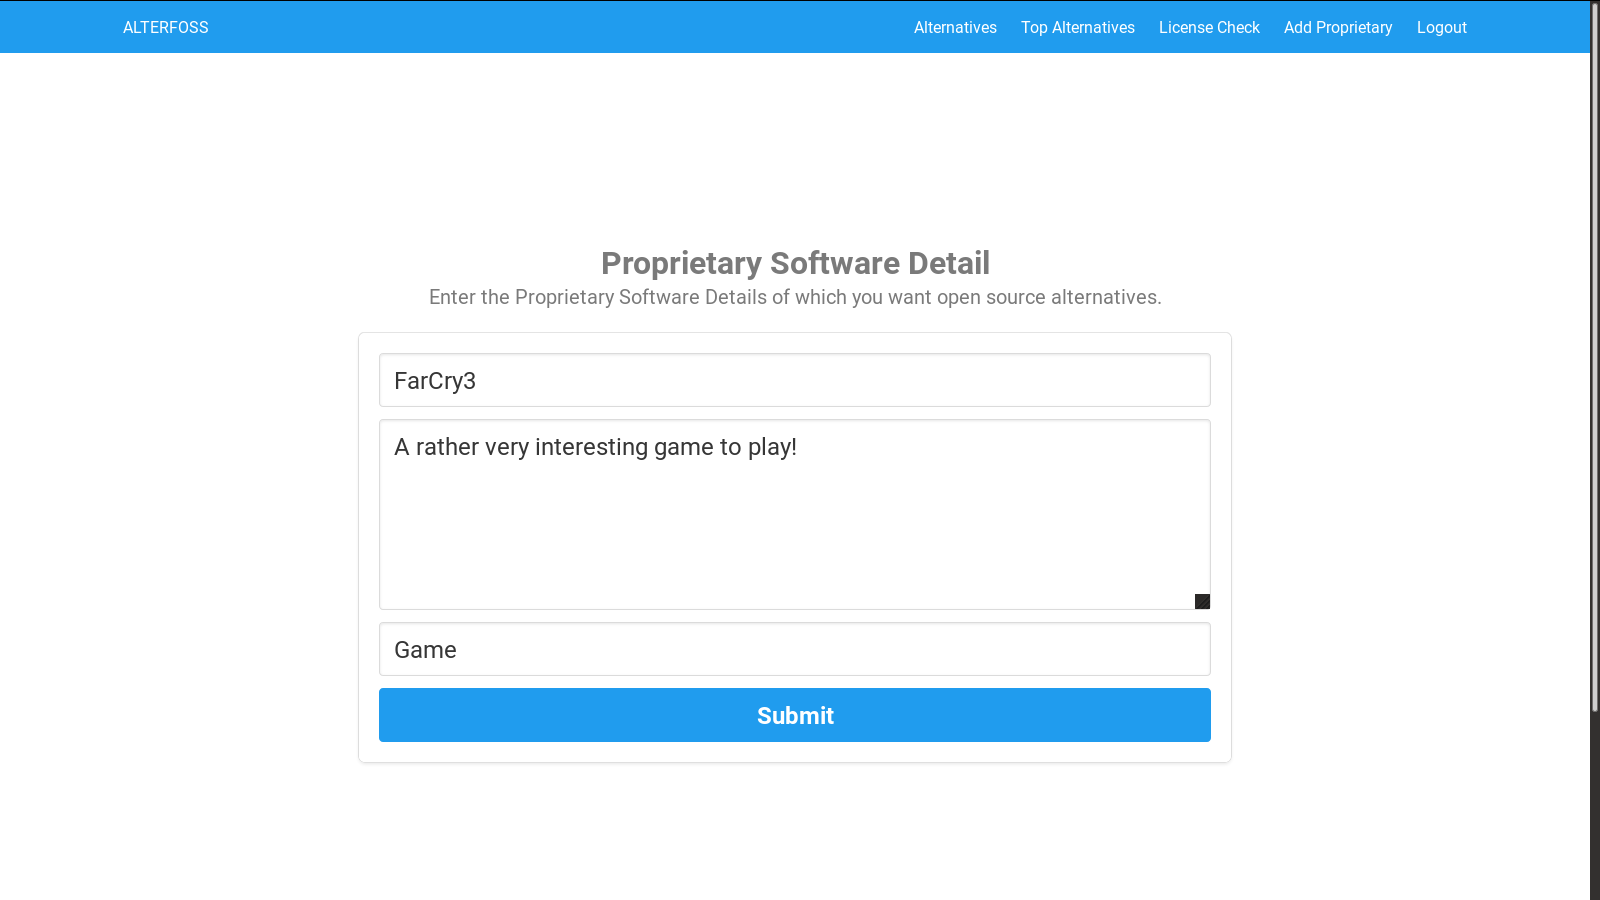
\includegraphics[scale=0.285]{images/4-6.png}
\caption{Adding a new proprietary software}
\label{fig:add_new_prop_sw}
\end{figure}

As can be seen in the Figure ~\ref{fig:add_new_prop_sw}, the user will have to provide the details of the software such as name, a short description, and tags via a form in order to request for this proprietary software's alternatives. The requested-by field will be set to anonymous automatically if the user is not logged in. Otherwise, the username will be fetched from the current session and will be assigned to the requested by field. A JSON object will be created using these details fetched from the user and this object is sent via the req.body property of the request. In response, the back-end will return the complete object written onto the database along with the \_id and \_v fields(though these can't be seen in the figure explicitly).


\begin{figure}[h!]
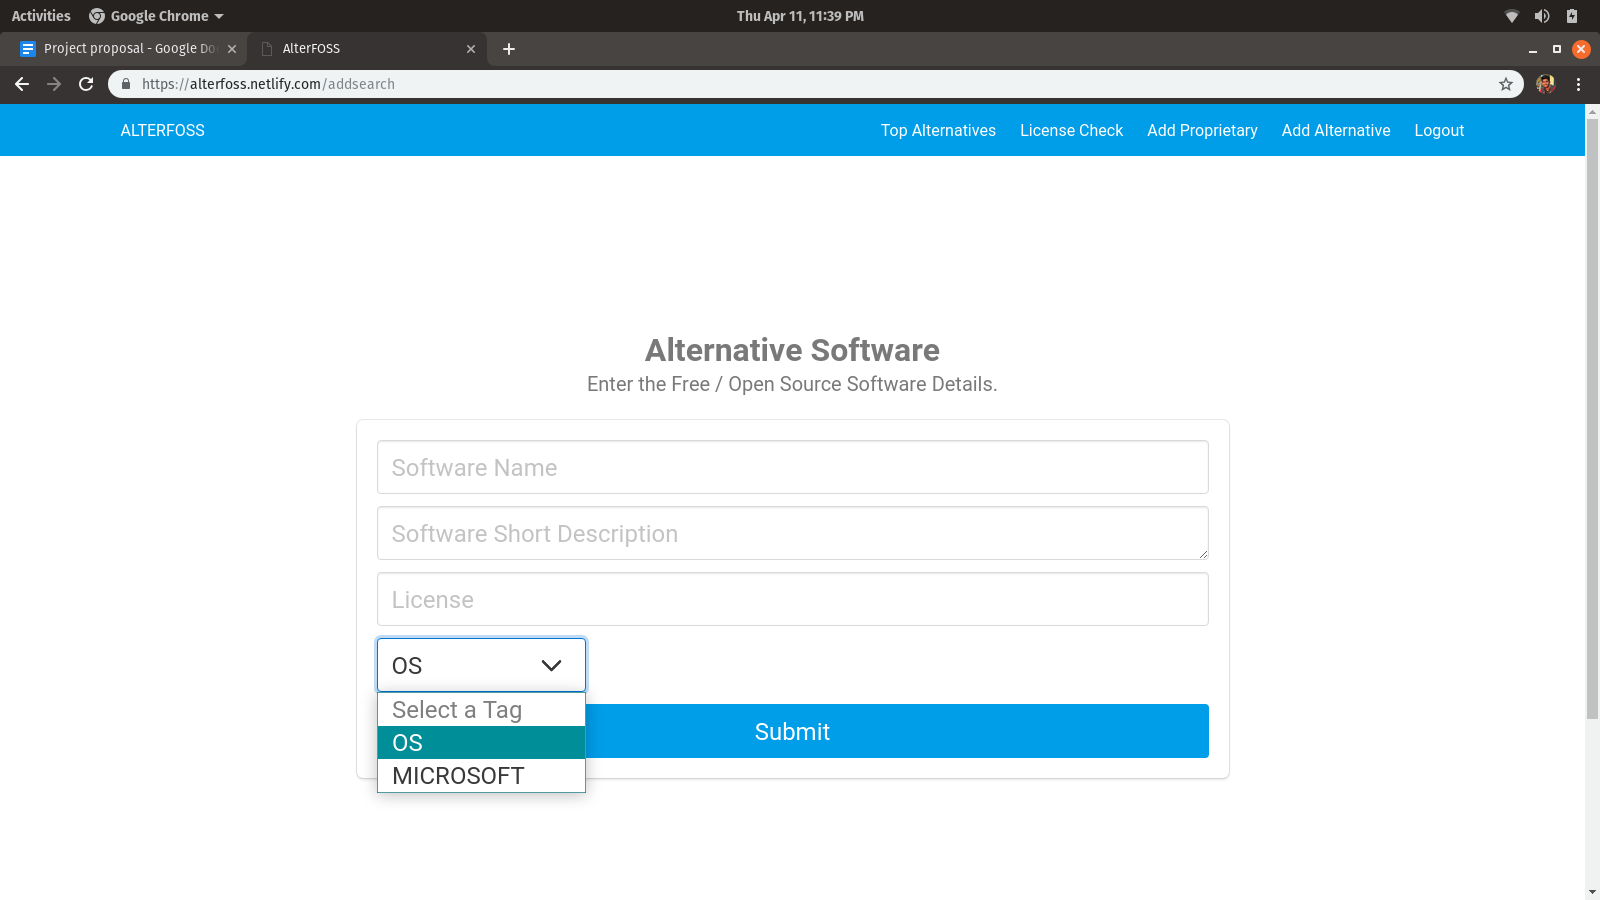
\includegraphics[scale=0.285]{images/4-7.png}
\caption{Creating a new alternative}
\label{fig:create_new_alt}
\end{figure}


Once the proprietary software is requested by someone as shown previously, the other community members will have the option to suggest alternatives for this proprietary software. This feature is also quite similar to that of the addition of proprietary software. The user needs to specify the name, license, short description and a handle for the alternative to be added. A JSON object is created using these properties and setting their values to those specified by the user via the front-end form. Here also, the suggested by field is set to the username from the current session, in case the user is logged in, otherwise, the default value ‘anonymous’ is used.

Both of these features to add an alternative and to create a proprietary software requires a ‘POST’ request to be sent to the server. These softwares are then stored inside the database and can be viewed by other users later. This way the platform will keep growing and the community will steer it.

\begin{figure}[h!]
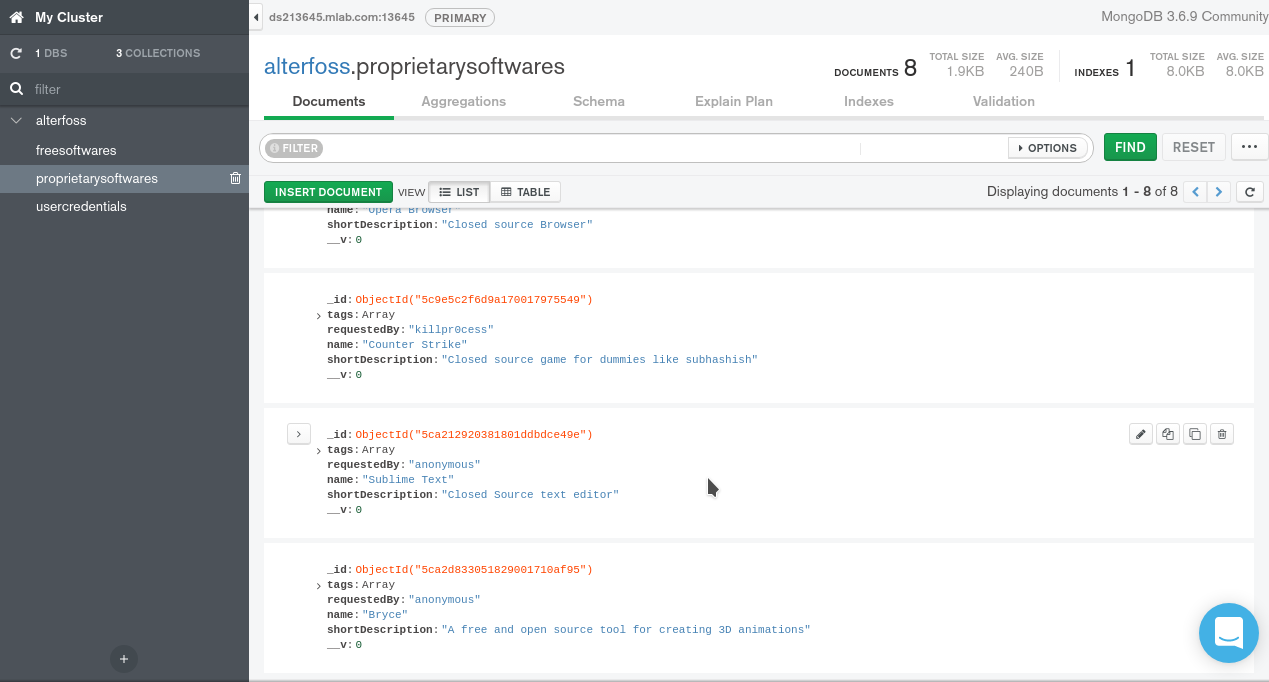
\includegraphics[scale=0.47]{images/4-8.png}
\caption{proprietarySoftware collections}
\label{fig:prop_db_collections}
\end{figure}

\begin{figure}[h!]
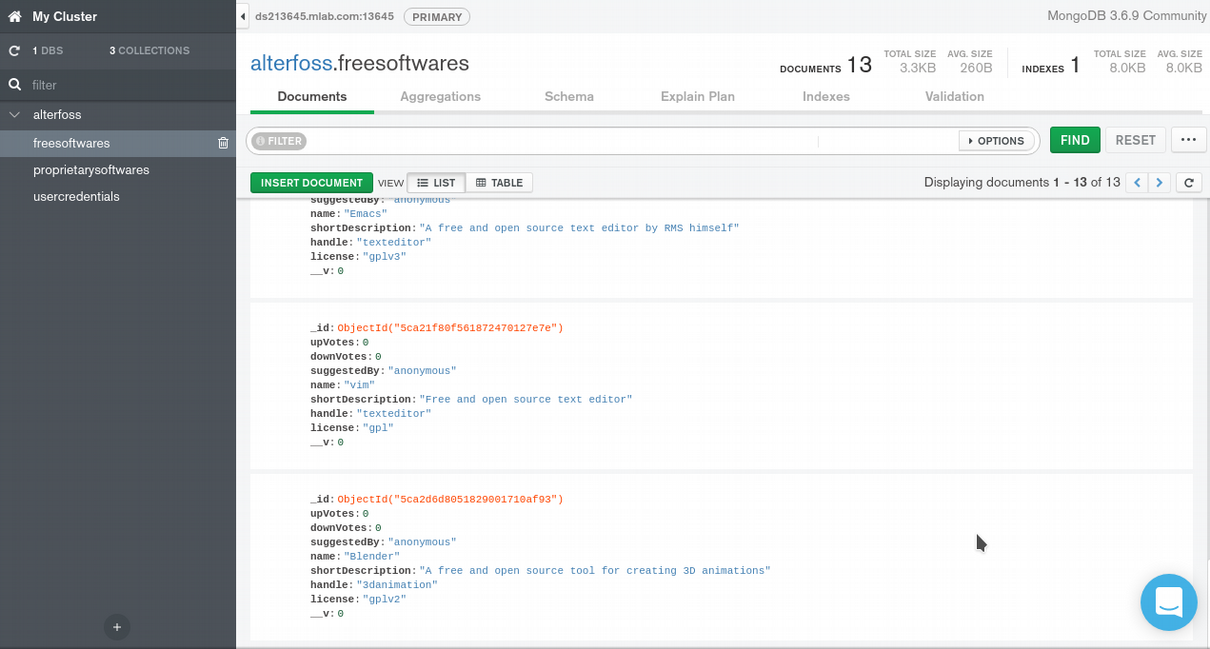
\includegraphics[scale=0.5]{images/4-9.png}
\caption{freeSoftwares collections}
\label{fig:fs_db_collections}
\end{figure}

The screenshots (Figure ~\ref{fig:prop_db_collections} and Figure ~\ref{fig:fs_db_collections}) show a glimpse of the database after the addition of these softwares.

\pagebreak
% ===================================================================================================
% END POINTS OF API
% ===================================================================================================
\section{RESTful API/End Points}

        
Each alternative software will be initialized with 0 upvotes and downvotes. These fields will be via \texttt{req.body.<field-name>}. If the \texttt{suggestedBy} field is not specified, then the default value is taken to be "\textsl{anonymous}". If the input syntax does not match this standard, the returned value is a string specifying the error.

\subsection{\texttt{GET Requests}}

\begin{itemize}

\item{\texttt{'GET' /}}

Home Page

\item{\texttt{'GET' /api/login/me}}

Used to query the database for user information. A token needs to be sent in the header of the request which shall then be verified. On successful verification, username, firstName, and lastName are returned in the response. Otherwise, a 400 error is raised.

\item{\texttt{'GET' /api/proprietary}}

Returns an array of all proprietary softwares as an array of objects.

\item{\texttt{'GET' /api/alternatives}}

Return an array of the top 10 alternatives (Free Softwares) as an array of objects containing the name, license, and upVotes for the softwares in decreasing order.

\item{\texttt{'GET' /api/alternatives/<id>}}

Returns the alternatives for the proprietary software specified by id. id has to be passed as argument in the URL.

\end{itemize}

\subsection{\texttt{POST Requests}}

\begin{itemize}

\item{\texttt{'POST' /api/alternatives}}

To add a new alternative to the free softwares. The body of the request contains the following fields:

\begin{itemize}
\item \texttt{name}: The name of the software
\item \texttt{shortDescription}: A one-line description of it
\item \texttt{handle}: A single keyword which will be used to assign it as an alternative
\item \texttt{license}: The software's license
\item \texttt{suggestedBy}: The username of the user who proposed this alternative
\end{itemize}

\item{\texttt{'POST' /api/proprietary/}}

This will add new proprietary software. Similar to adding alternative softwares, here also the request body must contain the following fields:
\begin{itemize}
\item \texttt{name}: name of the proprietary software
\item \texttt{shortDescription}: One line description of the software
\item \texttt{tags}: A string array consisting of strings that will be matched against the handle of the alternative softwares to verify it is an alternative
\item \texttt{requestedBy}: Username of the user who put up this proprietary software request
\end{itemize}

If the \texttt{requestedBy} field is not specified, then the default value is taken to be "\textsl{anonymous}". If the input syntax does not match this standard, the returned value is a string specifying the error.



\item{\texttt{'POST' /api/proprietary/}}

Used to search for proprietary softwares. The pattern will be used as a regular expression to search for proprietary softwares. Pass the search string the user enters to this endpoint. Returns an array of objects corresponding to the proprietary softwares matching the given search string. The string will be passed as a property 'search' inside the \texttt{req.body}.


\item{\texttt{'POST' /api/alternatives/license/}}

Used to search alternative softwares to check their license. Returns an array of objects containing the name of the alternatives matching the search property of the req.body object. The matching is done as regExp matching ignoring case.


\item{\texttt{'POST' /api/proprietary/search/}}

Used to search proprietary softwares. Returns an array of objects containing the name and shortDescription of the proprietary softwares matching the search property of the req.bodyobject. The matching is done as regExp matching ignoring case.


\item{\texttt{'POST' /api/signup}}

Used to sign-up a user onto the application. It takes user credentials in the request's body and then validates for correctness. If validation passes, the user is stored onto the database and automatically logged in. Additionally, a JSON web token is sent for future use. If the validation fails, the user is prompted with an appropriate error message.


\item{\texttt{'POST' /api/login}}

Used to log-in a user onto the application. There are two ways of doing it : 

\begin{enumerate}
\item \textbf{Through log-in credentials}: This method involves user sending in his username/email and password. On successful validation of the credentials, the user is logged onto the system as well as a JSON web token is sent for future use(session handling).

\item \textbf{Through JSON web token}: If a user queries with a valid JSON web token, he is logged onto the system after verifying the token's authenticity. Otherwise an \texttt{invalid-token} error is raised.
\end{enumerate}

\end{itemize}


\subsection{\texttt{PUT Requests}}

\begin{itemize}

\item{\texttt{'PUT' /api/alternatives/upvote/<id>}}
This will increase the number of upvotes for the given alternative software specified by id by 1. The id has to be passed as a parameter in the URL.


\item{\texttt{'PUT' /api/alternatives/unupvote/<id>}}
Will reduce the number of upvotes for the given alternative software specified by id by 1. The id has to be passed as a parameter in the URL. Automatically checks if the upvotes are already at 0, doesn’t do anything.


\item{\texttt{'PUT' /api/alternatives/downvote/<id>}}
This will increase the number of downvotes for the given alternative software specified by id by 1. The id has to be passed as a parameter in the URL.


\item{\texttt{'PUT' /api/alternatives/undownvote/<id>}}
Will reduce the number of downvotes for the given alternative software specified by id by 1. The id has to be passed as a parameter in the URL. Automatically checks if the upvotes is already at 0, doesn’t do anything.

\end{itemize}























